
% !TeX program = lualatex
% !TeX encoding = utf8
% !TeX spellcheck = uk_UA
% !BIB program = bibler

\documentclass[onlytextwidth]{beamer}
\usetheme{Electromagnetism}
\usepackage{Electromagnetism}
\usetikzlibrary{spy}
\hypersetup{
  colorlinks=true,
  linkcolor=cyan,  % Цвет для внутренних ссылок
  urlcolor=red,    % Цвет для URL
  citecolor=blue   % Цвет для библиографических ссылок
}



%\def\colform#1{
%    \tikz[baseline]{\node[fill=green!50, rectangle, anchor=base, font=\scriptsize]{#1}}
%}


%============================================================================
\title[Лекції електрики та магнетизму]{\huge\bfseries Магнітне поле у речовині}
\subtitle{Лекції з електрики та магнетизму}
\author{Пономаренко С. М.}
\date{}
%============================================================================
\graphicspath{{pictures/}}

\begin{document}


\begin{frame}[plain]
	\maketitle
	%	\tikz[remember picture,overlay] \node[opacity=0.7,inner sep=0pt,
	%		anchor=north west] at (current page.north
	%	west){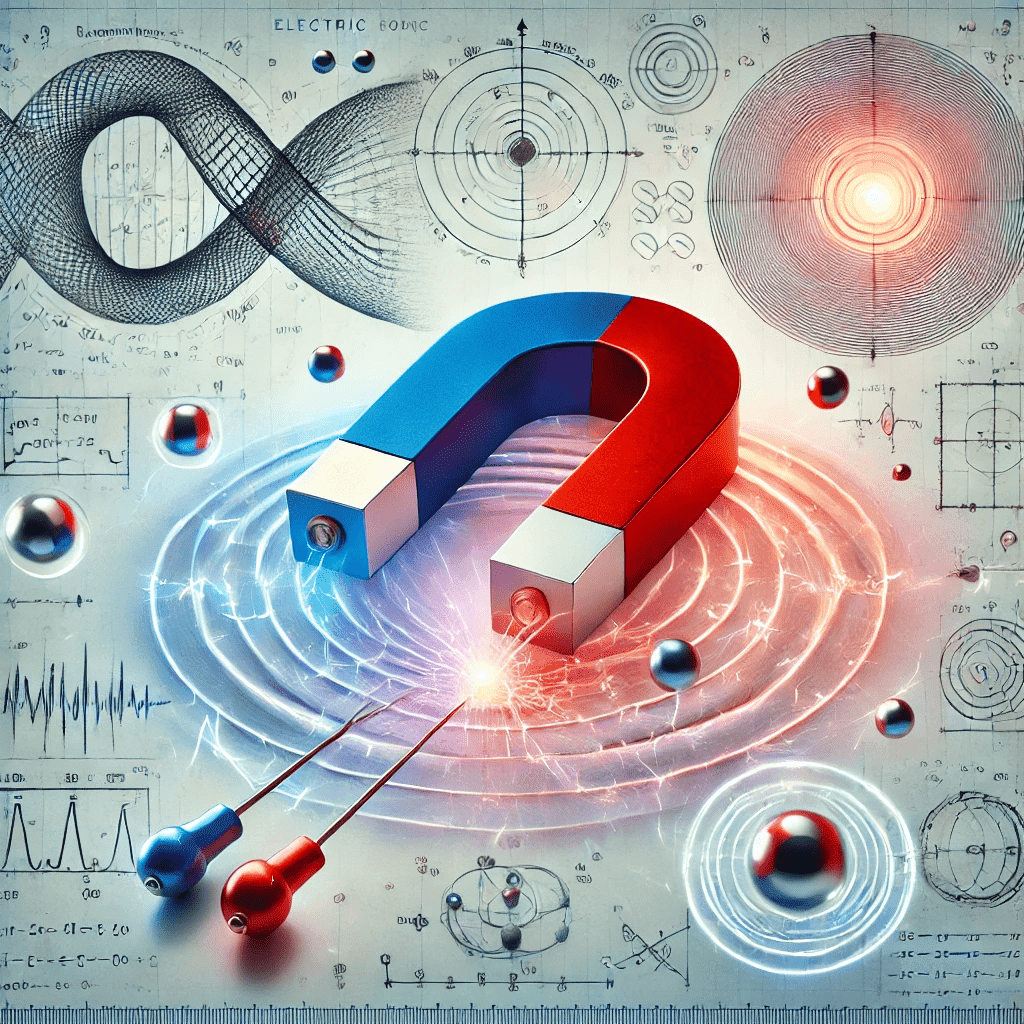
\includegraphics[width=2cm]{EMInteractions}};
\end{frame}

% ============================== Слайд ## ===================================
\begin{frame}{Зміст лекції}{}
	\tableofcontents
\end{frame}
% ===========================================================================


% ============================== Слайд ## ===================================
\begin{frame}{Гіпотеза Ампера}{Молекулярні струми}
	\begin{block}{}\justifying
		Якщо магнітне поле діє на рухомі заряджені частинки та рамки зі струмом, то \alert{чому воно також діє і на будь-який інший
			шматок магніту}? Ампер припустив, що \alert{всередині магніту теж течуть струми}.
	\end{block}


	\begin{block}{}\justifying\scriptsize
		Але якщо взяти стрілку або магніт у руки, то ніяких струмів ми не відчуваємо. Отже,  ці струми циркулюють усередині речовини і
		ніколи не виходять назовні. Що це за струми такі всередині речовини, Ампер звісно ж не знав. Сучасній науці вже відомо, що звичайна речовина
		складається з атомів. Своєю чергою, всередині атомів є позитивно заряджені ядра з негативно зарядженими електронами, що обертаються навколо них.
		Також самі електрони є маленькими магнітними стрілочками. Так
		ось, рух електронів усередині атомів є не що інше, як електричні струми, про існування яких припустив Ампер. Магнітне поле діє на ці струми, а
		значить і на речовину в цілому.
	\end{block}


	\begin{center}
		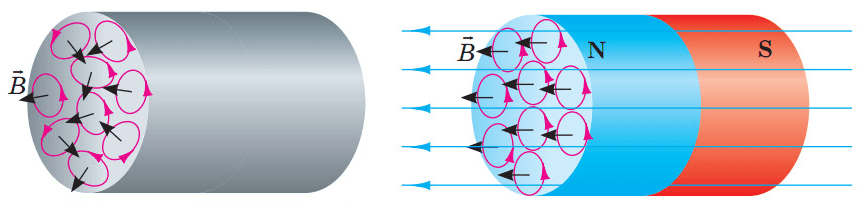
\includegraphics[width=1\linewidth]{AmpereHypotesis}
	\end{center}

\end{frame}
% ===========================================================================



% ============================== Слайд ## ===================================
\begin{frame}{Означення}{}
	\framesubtitle<1>{Мікрополе та середнє поле}
	\framesubtitle<2>{Струми провідності та молекулярні струми}
	\begin{onlyenv}<1>
		\begin{block}{}\justifying
			У речовині магнітне поле формується як зовнішнім полем, так і струмами, що циркулюють у цій речовині.

			\bigskip

			На мікрорівні (тобто на відстанях
			порядку розміру атомів і менше) поле різко змінюється в часі та просторі. Це поле називається \alert{мікрополем} $\Bfield_\text{micro}$ .
			Однак якщо провести усереднення за малим об'ємом, у якому є багато частинок (тобто за фізично нескінченно малим об'ємом), то отримаємо
			середнє поле:
			\begin{equation*}
				\left\langle \Bfield\right\rangle = \frac1{\Delta V} \iiint\limits_{\Delta V}
				\Bfield_\text{micro} dV.
			\end{equation*}
			\alert{Середнє поле} змінюється істотно повільніше внаслідок статистичного усереднення при випадковому русі частинок.
		\end{block}
	\end{onlyenv}
	\begin{onlyenv}<2>
		\begin{block}{}\justifying
			Створювані рухомими зарядами, можна розділити на дві групи: \alert{струми провідності} та \alert{молекулярні струми}.
			\begin{enumerate}
				\item \alert{Струми провідності} пов'язані з переміщенням вільних зарядів і є сторонніми щодо речовини.
				\item \alert{Молекулярні струми} зумовлені орбітальним рухом і спіном (власним моментом імпульсу) електронів в атомах (молекулах) і ядер речовини.
			\end{enumerate}
		\end{block}
	\end{onlyenv}
\end{frame}
% ===========================================================================


% ============================== Слайд ## ===================================
\begin{frame}{Вектор намагнічування}{}
	\begin{block}{}
		\alert{Вектор намагнічування} (або \alert{намагніченість}) — це величина, що характеризує магнітний момент одиниці об'єму речовини. Визначається вона
		як:

		\begin{equation*}
			\vect{J} = \frac{1}{V}\sum_i\vect{p}_i,
		\end{equation*}

		де $\vect{p}_i$ --- магнітні моменти окремих частинок.
	\end{block}


	\begin{block}{}\justifying\small
		Намагніченість називається \alert{однорідною}, якщо вектор $J$ не залежить від вибору точки в речовин. Якщо ж $\vect{J}\neq\const$, то
		намагніченість
		називається \alert{неоднорідною}.
	\end{block}
	\begin{center}
		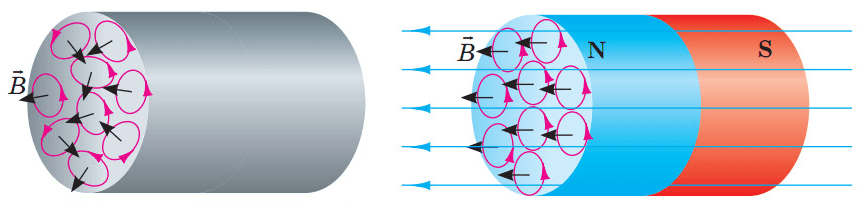
\includegraphics[width=1\linewidth]{AmpereHypotesis}
	\end{center}
\end{frame}
% ===========================================================================


% ============================== Слайд ## ===================================
\begin{frame}{Вимірювані величини і вилучення струмів намагнічення}{}
	\begin{alertblock}{Основна задача теорії магнітостатики в речовині}\justifying
		У магнітостатиці стоїть завдання знайти спосіб опису полів, які виникають через молекулярні струми, без їх безпосереднього обчислення.
		Основна ідея полягає у тому, щоб \textbf{вилучити} струми намагнічення з рівнянь і замінити їх іншими величинами, які можливо вимірювати
		безпосередньо, наприклад, вектором намагнічення $\vec{J}$.
	\end{alertblock}
	\begin{block}{Чому це важливо?}\justifying
		Виключення струмів намагнічення з розрахунків дозволяє зосередитись на вимірюваних параметрах, що спрощує математичні моделі. В результаті,
		обчислення магнітних полів у магнетиках стає доступнішим і більш наочним.
	\end{block}
\end{frame}
% ===========================================================================


% ============================== Слайд ## ===================================
\begin{frame}{Зв'язок намагніченості з молекулярними струмами}{}
	\begin{block}{}\justifying\scriptsize
		Виділимо в речовині досить малий циліндр, так що поле в ньому можна вважати практично однорідним. У його об'ємі молекулярні струми компенсують один
		одного. Циліндр (ліворуч) і вигляд його торця (праворуч). Кільцеві струми, що циркулюють в об'ємі, компенсують один одного всюди, окрім точок бічної
		поверхні. У результаті залишається тільки поверхневий струм, що тече бічною поверхнею циліндра.
	\end{block}
	\begin{columns}
		\begin{column}{0.5\linewidth}\centering
			\begin{tikzpicture}[>=latex]
				\draw[fill=gray!20] (0,0) arc(180:350:1 and 0.2) -- ++(45:2)  arc(350:180:1 and 0.2) -- cycle;
				\path (45:2) ++(1,0) coordinate (O);

				\begin{scope}[shift={(O)}, yscale=0.2]
					\draw[thick, blue, arrowpos={0.7}{2pt}{3pt}] (0,0) [partial ellipse=0:360:1];
					\foreach \a in {10, 40,...,340} {
							\draw[red, smooth, arrowpos={0.75}{2pt}{3pt}] (\a:0.8) [partial ellipse=0:360:0.2];
						}
					\foreach \a in {25,85,...,335} {
							\draw[red, smooth] (\a:0.42) [partial ellipse=0:360:0.2];
						}
					\draw[red, smooth] (0, 0) [partial ellipse=0:360:0.2];
				\end{scope}

				\foreach \l in {0.2,0.4,...,1.8} {
						\draw[blue, arrowpos={0.4}{2pt}{3pt}] (45:\l) arc(180:350:1 and 0.2);
					}
				\draw[->, ultra thick] (O) -- ++(0,1) coordinate (J) node[left] {$\vect{J}$};
				\draw (0,0) -- ++(0,2);
				\draw (0,0) ++(0, 0.5) arc (90:45:0.5) node[pos=0.5, anchor=south] {$\theta$};
				\draw[->] (O) -- ++(45:{1*cos(45)}) coordinate (Pr) node[right] {$\ell\vect{\tau}$};
				\draw[dashed] (J) -- (Pr);
				\draw[<->] (2.2, 0) -- node[right] {$\ell$} ++(45:2);
			\end{tikzpicture}
		\end{column}
		\begin{column}{0.5\linewidth}\centering
			\begin{tikzpicture}[>=latex]
				\draw[arrowpos={0.4}{2pt}{4pt}, thick, blue] (0,0) [partial ellipse=0:360:1.01];
				\foreach \a in {10, 40,...,340} {
						\draw[arrowpos={\a/360}{2pt}{3pt}, red] (\a:0.8) [partial ellipse=0:360:0.2];
					}
				\foreach \a in {25,85,...,335} {
						\draw[arrowpos={\a/360}{2pt}{3pt}, red] (\a:0.42) [partial ellipse=0:360:0.2];
					}
				\draw[arrowpos={0.5}{2pt}{3pt}, red] (0, 0) [partial ellipse=0:360:0.2];
			\end{tikzpicture}
		\end{column}
	\end{columns}
	\begin{block}{}\small
		Знайдемо магнітний момент такого циліндрика:
		\begin{equation*}
			\vect{p}_m = \vect{J}V = \frac1c I_mS\ \vect{n} \Rightarrow\ \vect{J}S\ell\cos\theta = \frac1c I_m S\ \vect{n}
			\Rightarrow\ \vect{J}\cdot\vect{\tau} \ell\cos\theta  = \frac1c I_m \ \vect{n}\cdot\vect{\tau}
		\end{equation*}
		\begin{equation*}
			{I_m}\ /\ {\ell} = i_m = c\vect{J}\cdot\vect{\tau},\ {\color{red}\vect{n}\cdot\vect{\tau} = \cos\theta}.
		\end{equation*}
		\alert{Молекулярні струми перпендикулярні намагніченості: $\vect{i}_m \perp \vect{J}$.}
	\end{block}
\end{frame}
% ===========================================================================





% ============================== Слайд ## ===================================
\begin{frame}{Циркуляція вектора намагнічення}{}
	\framesubtitle<2>{Молекулярні об'ємні струми намагнічення}
	\begin{onlyenv}<1>
		\begin{columns}
			\begin{column}{0.5\linewidth}
				\begin{tikzpicture}[>=latex, scale=0.85]
					\fill[red!20, draw=green!50!black, arrowpos={0.2}{0pt}{4pt}] (0,0) -- ++(4, 0) -- ++(-45:2) -- ++(-4, 0) --cycle;
					\foreach \x in {0,1,...,8}{
							\draw[arrowpos={0.45}{2pt}{3pt}, red, scale=0.5] (\x, 0) [partial ellipse=10:350:0.2 and 1];
							\draw[arrowpos={0.95}{2pt}{3pt}, red, scale=0.5] ({\x+3}, -2.8) [partial ellipse=10:350:0.12 and 0.6];
						}
					\draw[->, ultra thick, red!50, opacity=0.75] (2.8, -0.7) -- ++(0, -1.5) node[below] {$d\vect{S}$};
				\end{tikzpicture}
			\end{column}
			\begin{column}{0.5\linewidth}
				\begin{block}{}\justifying\small
					Виберемо тепер у речовині довільний замкнутий контур {\color{green!50!black}$L$}. На одиницю довжини контуру припадає струм
					намагнічування:
					\begin{equation*}
						i_m = c\vect{J}\cdot d\vect{\ell},
					\end{equation*}
					таким чином,  контур перетинає повний струм:
					\begin{equation*}
						I_m = c\oint\limits_L \vect{J}\cdot d\vect{\ell}.
					\end{equation*}
				\end{block}
			\end{column}
		\end{columns}
	\end{onlyenv}
	\begin{onlyenv}<1-2>
		\begin{block}{}\justifying
			Отриманий вираз на підставі теореми Стокса перетворюється на вигляд:
			\begin{equation*}
				I_m = c\oint\limits_L \vect{J}\cdot d\vect{\ell} = c \iint\limits_S \Rot\vect{J}\cdot d\vect{S}.
			\end{equation*}
			де $S$ --- поверхня, що спирається на контур $L$.
		\end{block}
	\end{onlyenv}
	\begin{onlyenv}<2>
		\begin{block}{}\justifying
			Струм, що протікає через поверхню $S$, виражається через густину струму формулою
			\(
			I_m = \iint\limits_S \vect{j}_m\cdot d\vect{S}.
			\)
			отже, що густина молекулярних струмів пов'язана з вектором намагнічування
			формулою:
			\begin{equation*}
				\tcbhighmath{\vect{j}_m = c\Rot\vect{J}.}
			\end{equation*}
			Це співвідношення дає \alert{зв'язок молекулярного струму з вектором намагнічування в диференціальній формі}.
		\end{block}
	\end{onlyenv}
\end{frame}
% ===========================================================================




% ============================== Слайд ## ===================================
\begin{frame}{Теорема про циркуляцію в речовині}{}
	\begin{onlyenv}<1>
		\begin{block}{}\justifying
			Циркуляцію магнітного поля породжують всі струми, як струми провідності так і струми намагнічування:
			\begin{equation*}
				\oint\limits_L\Bfield\cdot d\vect{\ell} = \frac{4\pi}c(I + I_m).
			\end{equation*}
			Тепер у нас є інструмент для вилучення $I_m$ з рівняння.
			\begin{equation*}
				\oint\limits_L\Bfield\cdot d\vect{\ell} = \frac{4\pi}c\left(I + c
				\iint\limits_S \Rot\vect{J}\cdot d\vect{S}\right).
			\end{equation*}
		\end{block}
	\end{onlyenv}
	\begin{onlyenv}<1-2>
		\begin{block}{}\justifying
			Введемо величину, що --- \alert{напруженість магнітного поля}:
			\begin{equation*}
				\tcbhighmath{\Hfield = \Bfield - 4\pi\vect{J}.}
			\end{equation*}
		\end{block}
	\end{onlyenv}
	\begin{onlyenv}<2>
		Теорема про циркуляцію в речовині прийме вигляд:
		\begin{columns}
			\begin{column}{0.5\linewidth}\centering
				\begin{equation*}
					\tcbhighmath{\oint\limits_L\Hfield\cdot d\vect{\ell} = \frac{4\pi}cI.}
				\end{equation*}
			\end{column}
			\begin{column}{0.5\linewidth}\centering
				\begin{equation*}
					\tcbhighmath{\Rot\Hfield = \frac{4\pi}c\vect{j}.}
				\end{equation*}
			\end{column}
		\end{columns}
		\begin{block}{}\justifying
			Вектор $\Hfield$ є допоміжним і слугує для спрощення вигляду рівнянь. Суттєво, що \alert{його циркуляція визначається тільки струмами провідності},
			що дає змогу в низці задач спростити розрахунок магнітного поля в середовищі.
		\end{block}
	\end{onlyenv}
\end{frame}
% ===========================================================================





% ============================== Слайд ## ===================================
\begin{frame}{Лінійні ізотропні магнітні середовища}{}
	\begin{block}{}
		Якщо магнітне поле слабке і в середовищі немає початкової намагніченості, то можна покласти:
		\begin{equation*}
			\vect{J} = \chi_m\Hfield.
		\end{equation*}
		Коефіцієнт $ \chi_m$ називається \alert{магнітною сприйнятливістю}.

		Підставимо це співвідношення у формулу $\Bfield = \Hfield + 4\pi\vect{J}$. Це дає
		\begin{equation*}
			\Bfield = (1+4\pi\chi_m)\Hfield = \mu\Hfield.
		\end{equation*}
		Величина $\tcbhighmath{\mu = 1+4\pi\chi_m}$ називається \alert{магнітною проникністю середовища}.
	\end{block}
\end{frame}
% ===========================================================================




% ============================== Слайд ## ===================================
\begin{frame}{Магнетики}{}\small
	\begin{block}{}\justifying
		Залежно від значення магнітної проникності виділяють такі основні класи середовищ:
		\begin{enumerate}
			\item Якщо $\chi_m > 0$, $\mu > 1$, то речовина називається \alert{парамагнетиком}. Парамагнітні властивості мають, наприклад,
			      \href{https://en.wikipedia.org/wiki/Aluminium}{\ce{Al}},
			      \href{https://en.wikipedia.org/wiki/Platinum}{\ce{Pt}},
			      \href{https://en.wikipedia.org/wiki/Iron(II)\_chloride}{\ce{FeCl2}},
			      \href{https://en.wikipedia.org/wiki/Oxygen}{\ce{O2}},
			      лужні та лужноземельні метали.

			\item Якщо $\chi_m < 0$, $\mu < 1$, то речовина називається \alert{діамагнетиком}. Діамагнетиками  є
			      \href{https://en.wikipedia.org/wiki/Bismuth}{\ce{Bi}},
			      \href{https://en.wikipedia.org/wiki/Antimony}{\ce{Sb}},
			      \href{https://en.wikipedia.org/wiki/Silicon}{\ce{Si}},
			      \href{https://en.wikipedia.org/wiki/Water}{\ce{H2O}},
			      \href{https://en.wikipedia.org/wiki/Dihydrogen}{\ce{H2}},
			      \href{https://en.wikipedia.org/wiki/Nitrogen}{\ce{N2}} тощо.
		\end{enumerate}
		Класифікація речовин на парамагнетики та діамагнетики запропонував М. Фарадей у 1845 р. Типові значення магнітної сприйнятливості для діа- і
		парамагнетиків становлять $|\mu| = 10^{-5} \div 10^{-5}$.
	\end{block}
	\vspace*{-1em}
	\begin{block}{}\justifying\footnotesize
		Деякі речовини можуть зберігати намагніченість $\vect{J}$ за відсутності зовнішнього магнітного поля. Для них не виконується просте співвідношення
		$\vect{J} = \chi_m\Hfield$ при всіх значеннях $\Hfield$. Такі речовини називаються \alert{феромагнетиками}. До їх числа належать, наприклад, \ce{Fe},
		\ce{Co}, \ce{Ni}. В діапазоні, де таке співвідношення формально виконується, магнітна проникність феромагнетиків сягає значень порядку $\mu
			\gg 1$.
	\end{block}
\end{frame}
% ===========================================================================




% ============================== Слайд ## ===================================
\begin{frame}{Задачі}{}
	\begin{exampleblock}{\scriptsize Задача 1}
		\begin{columns}
			\begin{column}{0.75\linewidth}\justifying\scriptsize
				Постійний струм $I$ тече вздовж довгого циліндричного дроту круглого перерізу. Дріт виготовлений з парамагнетика сприйнятливістю $\chi$.
				Знайти:
				\begin{enumerate}
					\item поверхневий молекулярний струм;
					\item об'ємний молекулярний струм.
				\end{enumerate}
				Як ці струми напрямлені один відносно одного?
				\bigskip

				\textit{Відповіді}:

				\begin{enumerate}
					\item $I'_\text{пов} = 4\pi\chi I$;
					\item $I'_\text{об} = 4\pi\chi I$.
				\end{enumerate}
				Струми напрямлені протилежно один відносно одного.

			\end{column}
			\begin{column}{0.25\linewidth}\centering
				\begin{tikzpicture}[>=latex]
					% Основные параметры
					\pgfmathsetmacro\h{3}          % Высота
					\pgfmathsetmacro\R{1}          % Радиус
					\coordinate (A) at (0, {-\h/2});
					\coordinate (B) at (0, {+\h/2});

					% Вертикальные линии
					\draw[gray] ([xshift=\R cm]A) -- ([xshift=\R cm]B)
					([xshift=-\R cm]A) -- ([xshift=-\R cm]B);
					\draw[line width={\R*2cm}, gray!50] (A) -- (B);

					% Верхняя и нижняя части
					\draw[gray, fill=gray!50] (B) circle ({\R} and {0.2*\R});
					\draw[gray] ([xshift=\R cm]A) arc(0:-180:{\R} and {0.2*\R});
					\draw[gray, densely dashed] ([xshift=-\R cm]A) arc(180:0:{\R} and {0.2*\R});
					\fill[gray!50] (A) circle ({\R} and {0.2*\R});

					% Стрелка для тока
					\draw[->] ([yshift={\h*0.3cm}]A) -- ([yshift={-\h*0.3cm}]B) node[above] {$I$};

					% Параметры для витков
					\def\fLarge{0.8}  % Масштаб большого витка
					\def\fSmall{0.4}  % Масштаб маленького витка

					% Витки на разных уровнях
					\foreach \y in {-1.5, -1, ..., +1.5} {
							\pgfmathtruncatemacro{\c}{round(\y)}
							\ifnum\c=0 \edef\t{1} \else \edef\t{0.1} \fi % Прозрачность
							\begin{scope}[opacity=\t]

								% Большой виток
								\draw[arrowpos={0.4}{0}{3pt}, blue] (0,{0.8*\y})
								[partial ellipse=91:{360+89}:{\fLarge*\R} and {\fLarge*0.2*\R}];
								\draw[arrowpos={0.5}{2pt}{3pt}, green!50!black] (0,{0.8*\y})
								++(180:{\fLarge*\R}) circle(0.2);
								\draw[arrowpos={0}{2pt}{3pt}, green!50!black] (0,{0.8*\y})
								++(0:{\fLarge*\R}) circle(0.2);

								% Маленький виток
								\draw[arrowpos={0.4}{0}{2pt}, blue] (0,{0.8*\y})
								[partial ellipse=91:{360+89}:{\fSmall*\R} and {\fSmall*0.2*\R}];
								\draw[arrowpos={0.5}{1.2pt}{2pt}, green!50!black] (0,{0.8*\y})
								++(180:{\fSmall*\R}) circle(0.1);
								\draw[arrowpos={0.5}{1.2pt}{2pt}, green!50!black, rotate=180] (0,{0.8*\y})
								++(180:{\fSmall*\R}) circle(0.1);
							\end{scope}
						}
				\end{tikzpicture}
			\end{column}
		\end{columns}

	\end{exampleblock}
\end{frame}
% ===========================================================================


% ============================== Слайд ## ===================================
\begin{frame}{Граничні умови для $\Bfield$ та $\Hfield$}{}
	\begin{onlyenv}<1>
		\begin{columns}
			\begin{column}{0.6\linewidth}
				\begin{block}{}\scriptsize\justifying
					Застосуємо теорему Гауса до нескінченно малого циліндра, що охоплює частину межі
					розділу двох
					середовищ. Вважаючи $d\vect{S}_1 = - d\vect{S}_2$, $q = \sigma dS$,
					$d\vect{S}_1 =
						\vect{n}\ dS$,
					маємо
				\end{block}
			\end{column}
			\begin{column}{0.4\linewidth}\centering
				 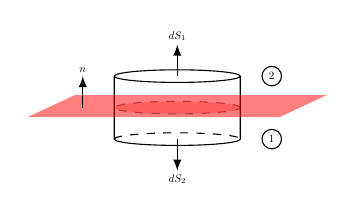
\begin{tikzpicture}[
scale=0.4,
transform shape,
>=latex,
declare function = {
h = 2;
r=2;
r2=0.2;
},
]

\fill[red!50, opacity=0.5, draw=black, dashed] (0,1) circle (r and r2);
\draw (-2,h) -- (-2,0) arc (180:360:r and r2) -- (2,h) ++ (-2,0) circle (r and r2);
\draw[dashed] (-2,0) arc (180:0:r and r2);
\fill[red,opacity=0.5]
 (-4.75,0.7) -- ++(8,0) -- ++(1.5,0.7) -- ++(-8,0) ;
\draw[->] (0,h) -- ++(0,1) node[above] {$d\vect{S}_1$};
\draw[->] (0,0) -- ++(0,-1) node[below] {$d\vect{S}_2$};

\draw[->] (-3,1) -- ++(0,1) node[above] {$\vect{n}$};

\node[circle, draw] at (3,0) {$1$};
\node[circle, draw] at (3,h) {$2$};
\end{tikzpicture}
			\end{column}
		\end{columns}
		\begin{block}{}\scriptsize
			\begin{equation*}
				\oiint_S \Bfield_1\cdot d\vect{S} = 0\ \Rightarrow  \Bfield_2\cdot
				d\vect{S}_1 +
				\Bfield\cdot d\vect{S}_2 = 0
			\end{equation*}
		\end{block}
		\begin{block}{}
			Звідси випливає перша гранична умова:
			\begin{equation*}
				\tcbhighmath{
					B_{1n} = B_{2n}.
				}
			\end{equation*}
		\end{block}
		\begin{alertblock}{}\justifying\scriptsize
			Нормальна складова вектора $\Bfield$ не зазнає стрибка при
			переході через границю розділу середовищ.
		\end{alertblock}
	\end{onlyenv}
	\begin{onlyenv}<2>
		\begin{columns}
			\begin{column}{0.6\linewidth}
				\begin{block}{}\scriptsize\justifying
					Застосуємо теорему про циркуляцію до нескінченно малого прямокутного
					контуру $L$, що проходить на нескінченно малій відстані над і під поверхнею
					розділу середовищ. Вважаючи, що $d\vect{r}_1 = -d\vect{r}_2$, маємо
				\end{block}
			\end{column}
			\begin{column}{0.4\linewidth}\centering
				 \begin{tikzpicture}[
scale=0.4,
transform shape,
>=latex,
declare function = {
h = 2;
r=2;
r2=0.2;
},
midarrow/.style={%
   postaction={ decorate,transform shape,
   decoration={ markings, mark=at position .5 with {\arrow{>}}}}},
]

\fill[red,opacity=0.5]
 (-4.75,0.7) -- ++(8,0) -- ++(1.5,0.7) -- ++(-8,0) ;

\draw[midarrow] (2, 1) -- ++(0, 1) -- node[above=5pt] {$L$} ++(-4, 0) -- ++(0, -1);
\draw[midarrow] (-2, 1) -- ++(0, -1) -- ++(4, 0) -- ++(0, 1);

\draw[->] (-3,1) -- ++(-2,0) node[above] {$\vect{\tau}$};
\draw[->] (-3,1) -- ++(0,1) node[above] {$\vect{n}$};
\draw[->] (-3,1) -- ++({180+45}:1) node[below] {$\vect{b}$};
\node[circle, draw] at (3,0) {$1$};
\node[circle, draw] at (3,h) {$2$};
\end{tikzpicture}
			\end{column}
		\end{columns}
		\begin{block}{}\scriptsize
			\begin{equation*}
				\oint\limits_L \Hfield\cdot d\vect{r} = \frac{4\pi}cI \Rightarrow \Hfield_1 d\vect{r}_1 +
				\Hfield_2 d\vect{r}_2 = \frac{4\pi}c i_b d\ell
			\end{equation*}
		\end{block}
		\begin{block}{}
			Звідси випливає друга гранична умова:
			\(
			\tcbhighmath{
				H_{2\tau} - H_{1\tau} = \frac{4\pi}c i_b.
			}
			\)
		\end{block}
		\begin{block}{}\justifying\scriptsize
			Останню умову можна можна записати у векторному вигляді: Оскільки $ \vect{\tau} = \vect{b}\times\vect{n} $. То $(\Hfield_2 - \Hfield_1)\vect{\tau} =
				\frac{4\pi}c i_b $, або $(\Hfield_2 - \Hfield_1)[\vect{b}\times\vect{n}] = \frac{4\pi}c i_b $. Зробивши циклічний зсув співмножників у змішаному
			добутку векторів, отримаємо:
			\(
			\tcbhighmath{
				\vect{n}\times (\Hfield_2 - \Hfield_1) = \frac{4\pi}c \vect{i}.
			}
			\)
		\end{block}
		\begin{alertblock}{}\centering\scriptsize
			Тангенціальна складова $\Hfield$ зазнає розриву, якщо по поверхні розділу середовищ течуть \alert{струми провідності}.
		\end{alertblock}
	\end{onlyenv}
\end{frame}
% ===========================================================================





% ============================== Слайд ## ===================================
\begin{frame}{Заломлення силових ліній на границі магнетиків}{}\small
	\begin{block}{}\justifying
		Лінії векторів $\Bfield$ і $\Hfield$ на границі розділу двох
		магнетиків заломлюються.
	\end{block}
	\begin{columns}
		\begin{column}{0.55\linewidth}\centering
			\begin{tikzpicture}[>=latex,
					scale=0.73,
					transform shape,
					pencildraw/.style={ %
							decorate,
							decoration={random steps,segment length=3pt,amplitude=2pt}
						},
				]



				% Георметрія

				% Середовище 1
				\fill[thick, red!10,  pencildraw, opacity=0.85] (-2, +0.05) rectangle (6, -2.1);
				\node[circle, draw, inner sep =1pt, font=\scriptsize] at (-1.8, -0.5) {$1$};

				% Середовище 2
				\fill[thick, blue!10, pencildraw, opacity=0.85] (-2, -0.05) rectangle (6, +2.1);
				\node[circle, draw, inner sep =1pt, font=\scriptsize] at (-1.8, +0.5) {$2$};

				% Границя розділу
				\draw[line width=2pt, gray!50] (-2, 0) -- (6, 0);

				\draw[dashed] (-1, -2) -- ++(0, 4);

				\draw[midarrow] (-1.5, -2) -- (-1,0);
				%				\draw[->, red, thin, opacity=0.5] (-1.5, 0) -- node[above, font=\scriptsize]
				%				{$E_{1\tau}$}
				%				++(0.5, 0);
				%				\draw[->, red, thin, opacity=0.5] (-1.5, -2) -- node[left, font=\scriptsize]
				%				{$E_{1n}$} ++(0, 2);
				%
				%				\draw[->, red, thin, opacity=0.5] (-1, 0)     -- node[above, font=\scriptsize]
				%				{$E_{2\tau}$}
				%				++(1, 0);
				%				\draw[->, red, thin, opacity=0.5] (0, 0)      -- node[right, font=\scriptsize]
				%				{$E_{2n}$} ++(0,
				%				2);

				\draw[midarrow] (-1,0) -- ++(1, 2);
				\draw (-1,0) ++(90:0.8) arc[start angle=90, delta angle={-atan(1/2)}, radius =
						0.8]  node[pos=0.5, anchor=south, inner sep=1, font=\scriptsize] {$\alpha_2$};
				\draw (-1,0) ++(-90:0.8) arc[start angle=-90, delta angle={-atan(0.5/2)}, radius =
						0.8] node[pos=0.5, anchor=north, inner sep=5pt, font=\scriptsize] {$\alpha_1$};

				% Поле вектора E
				\foreach[] \x in {0,1,...,6}{
						\draw[midarrow, red] (0.25*\x, -2) -- ++(0.5, 2);
						\ifnum\x<4
							\draw[midarrow, red] ({0.5*(\x + 1)}, 0) -- ++(1, 2);
						\fi
					}
				\node[font=\small] at (0.8, -2.5) {Поле вектора $\Hfield$};

				% Поле вектора D
				\begin{scope}[xshift=3cm]
					\foreach[] \x in {0,1,...,6}{
							\draw[midarrow, blue ] (0.25*\x, -2) -- ++(0.5, 2);
							\draw[midarrow, blue ] ({0.25*(\x+2)}, 0) -- ++(1, 2);
						}
				\end{scope}
				\node[font=\small] at (3.8, -2.5) {Поле вектора $\Bfield$};

			\end{tikzpicture}
		\end{column}
		\begin{column}{0.45\linewidth}\scriptsize
			Граничні умови для вектора $\Hfield$
			\begin{equation*}
				\begin{cases}
					H_{1\tau} = H_{2\tau},\ \Rightarrow\ H_1\sin\alpha_1 = H_2\sin\alpha_2, \\
					B_{1n} = B_{2n},\ \Rightarrow\ \mu_1H_1\cos\alpha_1 =
					\mu_2H_2\cos\alpha_2
				\end{cases}
			\end{equation*}
			Граничні умови для вектора $\Bfield$
			\begin{equation*}
				\begin{cases}
					H_{1\tau} = H_{2\tau},\ \Rightarrow\ B_1/\mu_1\sin\alpha_1 =
					B_2/\mu_2\sin\alpha_2, \\
					B_{1n} = B_{2n},\ \Rightarrow\ B_1\cos\alpha_1 =
					B_2\cos\alpha_2
				\end{cases}
			\end{equation*}
		\end{column}
	\end{columns}
	\begin{block}{}\justifying
		Закон заломлення ліній $\Bfield$ та $\Hfield$ однаковий:
		\begin{equation*}
			\tg\alpha_2 / \tg\alpha_1 = \mu_2 / \mu_1.
		\end{equation*}
		В діелектрику з більшим значенням $\mu$ лінії $\Hfield$ і $\Bfield$
		становитимуть більший кут із нормаллю до границі розділу.
	\end{block}
\end{frame}
% ===========================================================================



% ============================== Слайд ## ===================================
\begin{frame}{Магнітне екранування}{}
	\begin{block}{}\justifying
		На заломленні магнітних ліній заснований \alert{магнітний захист}.
	\end{block}
	\begin{columns}
		\begin{column}{0.5\linewidth}
			\begin{block}{}\justifying\small
				При внесенні, наприклад, замкненої залізної оболонки (шару) в зовнішнє магнітне
				поле лінії цього поля будуть концентруватися (згущуватися) переважно в самій оболонці. Усередині ж цієї оболонки --- в порожнині --- магнітне поле
				виявляється сильно ослабленим порівняно із зовнішнім полем. Іншими словами, \alert{залізна оболонка має екрануючу дію}.
			\end{block}
		\end{column}
		\begin{column}{0.5\linewidth}\centering
			\includegraphics[width=0.75\linewidth]{magshield}
		\end{column}
	\end{columns}
	\begin{block}{}
		Це використовують для
		оберігання чутливих  приладів від зовнішніх магнітних полів.
	\end{block}
\end{frame}
% ===========================================================================



% ============================== Слайд ## ===================================
\begin{frame}{Феромагнетики}{}
	\begin{block}{}
		\alert{Феромагнетиками} називають речовини (тверді), які можуть мати \alert{спонтанну намагніченість в середині окремих доменів}, тобто
		намагнічені вже за відсутності зовнішнього магнітного поля. Типові представники феромагнетиків --- це залізо, кобальт і багато їхніх сплавів.
	\end{block}
	\begin{columns}
		\begin{column}{0.65\linewidth}
			\begin{block}{}\justifying\small
				\alert{Домен} --- це локальна область усередині феромагнетика, де дипольні моменти
				орієнтовані в одному й тому самому напрямку. У кожному домені намагніченість постійна і спрямована
				в один бік.
			\end{block}
		\end{column}
		\begin{column}{0.3\linewidth}\centering
			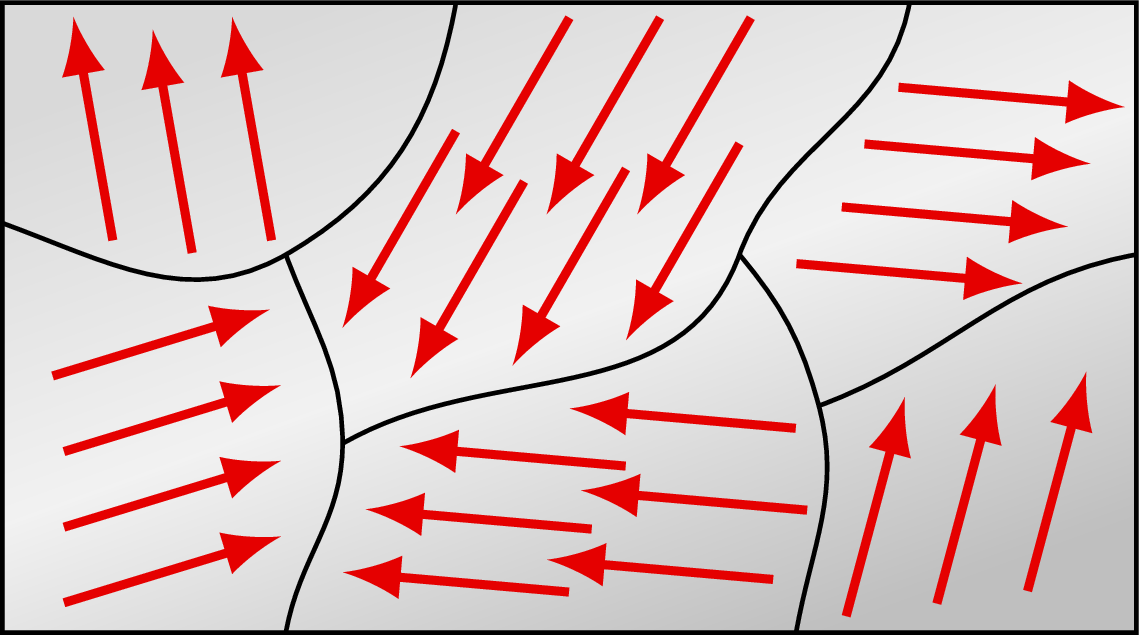
\includegraphics[width=1\linewidth]{domains}
		\end{column}
	\end{columns}
\end{frame}
% ===========================================================================


% ============================== Слайд ## ===================================
\begin{frame}{Гістерезис в феромагнетиках}{}\small
	\begin{block}{}\justifying
		\alert{Гістерезис} --- неоднозначна петлеподібна залежність поляризації сегнетоелектриків від
		зовнішнього магнітного поля $\Hfield$ за його циклічної зміни.
	\end{block}
	\begin{columns}
		\begin{column}{0.5\linewidth}\centering
			\begin{tikzpicture}[>=latex, scale=0.8, transform shape,
					point/.style={circle, draw, inner sep=0.7pt, fill=white}
				]

				\draw[-latex, name path=E] (-2.5,0) -- (2.5,0) node[below]{$H$};
				\draw[-latex, name path
					=P] (0,-1.5) -- (0,1.5)node[left]{$J $};

				\draw[samples=200, domain=-3:2, name path=d, midarrow,  red, thick] plot ({\x+0.5}, {0.2*\x
						+ tanh(1.9*\x) + 0.1}); \draw[samples=200, domain=-2:3, name path=u, midarrowR, red, thick]
				plot ({\x-0.5}, {0.2*\x + tanh(1.9*\x) - 0.1});
				\draw[midarrow, thick, cyan!50!black] (0,0) .. controls (0.5, 0.2) and
				(0.2, 1.0) ..
				(1.52, 1.28);
				\tikzfillbetween[of=u and d]{blue, opacity=0.1};

				\foreach \i/\a in {P/u, P/d, E/u, E/d} {
						\path[name intersections={of={\i} and {\a}}]
						(intersection-1) node[point] (\i\a) {};
					}
				\node[left,  text=brown] at (Pu) {$J_r$};
				\node[right, text=brown] at (Pd) {$-J_r$};
				\node[above left, text=red] at (Eu) {$-H_c$};
				\node[below right, text=red] at (Ed) {$H_c$};
			\end{tikzpicture}
		\end{column}
		\begin{column}{0.5\linewidth}
			\begin{figure}
				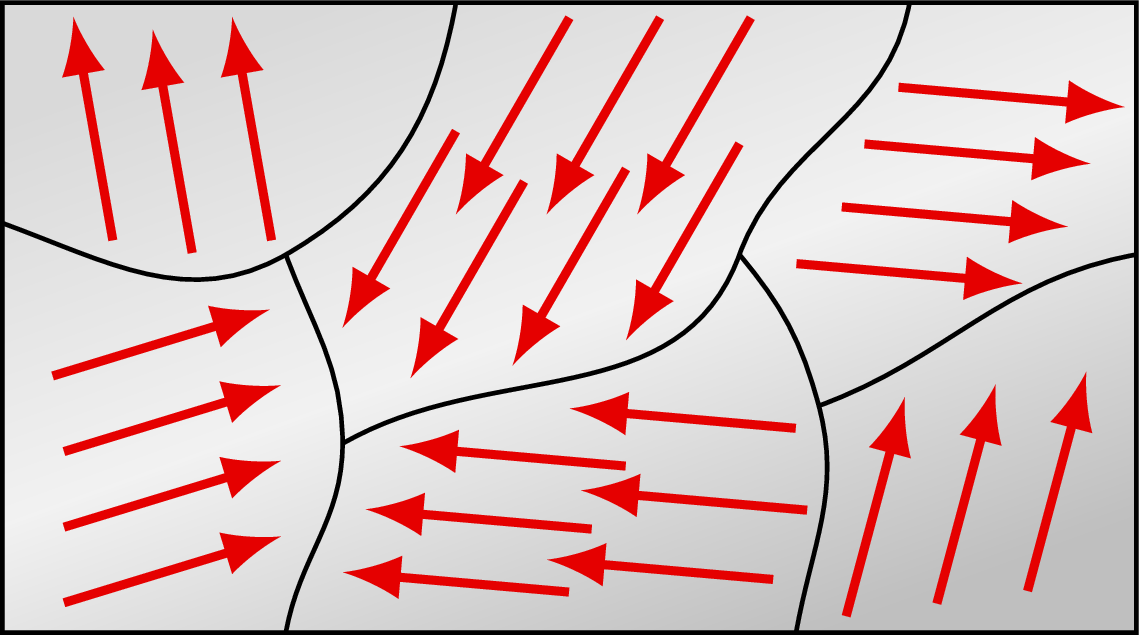
\includegraphics[width=0.5\linewidth]{domains}
				\caption{\centering\scriptsize Доменна структура феромагнетика}
			\end{figure}
		\end{column}
	\end{columns}
	\begin{enumerate}\justifying\scriptsize
		\item За високого поля $ H $, намагніченість досягає насичення і поводить себе як
		      парамагнетик у якого $J \propto H$.
		\item  Поле зменшується до нуля $H = 0$, але намагніченість $ J_r $ залишається.
		\item Для того щоб звести намагніченість до нуля, потрібно прикласти негативне поле $-H_c$,
		      яке називається \alert{коерцитивною силою}.
		\item При подальшому збільшенні негативного поля намагніченість $J \propto H$.
		\item  При зменшенні негативного поля до нуля намагніченість залишається на рівні $ -J_r $.
	\end{enumerate}
\end{frame}
% ===========================================================================



% ============================== Слайд ## ===================================
\begin{frame}{Магнітом'які та магнітожорсткі феромагнетики}{}
       \begin{block}{}\justifying
\alert{Магнітом'який} матеріал, який застосовують як осердя в трансформаторах, електромагнітах та інших приладах і машинах, характерний дуже вузькою
петлею гістерезису. Вузькість петлі (мала коерцитивна сила) означає малі втрати на перемагнічування. У ділянці до насичення петля близька до прямої
лінії, рівняння якої можна записати, як для неферомагнітних речовин, у вигляді $\Bfield = \mu\Hfield$.
\end{block}

\begin{block}{}\justifying
Постійні магніти слід виготовляти з магнітно-жорстких матеріалів, наприклад із загартованої сталі. Гістерезисна петля її широка, $H_c$ велика, що
забезпечує стійкість намагнічування.
\end{block}
\end{frame}
% ===========================================================================

\end{document}
